\documentclass[sigconf]{acmart}

% Blind-draft scaffold for TKDE submission.
% Sections 1-10 fully drafted (code-anchored); numbers in §3-§7 verified
% against frozen runs; figures/tables in §8-§9 use frozen results.
\title{Declarative Evidence Execution for Multi-Hop RAG:\\ Requirement-Aware
Physical Optimization under Matched Budgets}

\author{Anonymous}
\affiliation{%
  \institution{Anonymous Institution}
  \country{}
}
\email{anonymous@anonymous.edu}

\usepackage{booktabs}
\usepackage{multirow}
\usepackage{bm}
\usepackage{lmodern}

% \code: typeset a code identifier (replaces inline \verb to keep 1-line safe).
\newcommand{\code}[1]{\texttt{#1}}

\begin{document}

\begin{abstract}
Multi-hop retrieval-augmented generation (RAG) requires acquiring mutually
dependent evidence items under finite resource budgets before producing an
answer. We treat this as an \emph{execution} problem: a question is compiled
into a typed evidence program whose requirements are first-class objects with
status, type, importance, and dependencies; a deterministic importance-weighted
allocator assigns execution orders, physical implementations, and budget
allocations to those requirements under a matched budget; and a
deterministic adaptive executor acquires evidence, enforces budgets, and
records provenance. We derive a chain law that pins requirement importance to
dependency depth ($\tau = 2d-1$) on well-defined chains, making the estimator
construction-derived rather than learned. Under the matched-budget protocol on
three multi-hop QA workloads (HotpotQA, 2WikiMultiHopQA, MuSiQue; $55$ matched
questions), the requirement-aware allocator does not spend more on average than
the frozen static baseline on the matched valid pairs---pooled $-0.16$ calls/question, with EM differences
directionally positive on all three datasets ($\Delta$EM $+6.3/+5.9/+9.1$pt)
---though neither effect is statistically supported at this sample size
(cost bootstrap $p\in[0.119,0.376]$; EM McNemar $p\geq0.625$), and we report
both as such. On the $\ge 3$-slot subdomain, where the chain law gives the
allocator genuine freedom, the cost saving is larger and statistically
supported in the cleanest comparison: pooled $3.45$ calls/question versus
$4.73$ for the cost-only arm ($\Delta=-1.27$, bootstrap $p<0.001$; vs.\
static $-1.09$, $p=0.036$), at pooled EM that is equal across arms
($54.5\%/45.5\%/54.5\%$). We state the structural boundary honestly: on the
$1$--$2$-slot chains that dominate most QA splits, a budget floor leaves the
optimizer little allocation freedom.
\end{abstract}

\maketitle

% --- Section order per LOOP_PROMPT writing map ---
\section{Introduction}
\label{sec:intro}

Retrieval-augmented generation (RAG) decomposes complex questions into
retrieval and reasoning steps, and a growing line of work makes those steps
increasingly explicit: logical query trees \cite{planrag}, executable programs
\cite{pyrag}, typed slots \cite{slotrag}, and learned adaptive control
\cite{dynakrag}. This explicitness is a prerequisite for treating multi-hop
retrieval as an \emph{execution} problem rather than a prompt-engineering
problem. But it also raises a systems question that most RAG papers do not
state precisely: given a finite resource budget, \emph{how should a system
compile a question into dependent evidence requirements, choose physical
implementations for them, allocate budget across them, and acquire the evidence
while observing the outcomes at runtime}?

This paper answers that question with a concrete evidence-centric execution
model. We make three connected moves. First, we treat evidence \emph{requirements}
--- conditions that must be satisfied, with a type, an importance, a set of
variables to bind, and dependencies over other requirements --- as first-class
objects, and give them a typed algebra with monotone state-transition
semantics (\S\ref{sec:algebra}). Second, we separate the logical evidence
program from its physical implementations and introduce a deterministic
importance-weighted allocator that assigns execution orders, retrieval
implementations, and budget allocations to typed requirements under a matched
budget (\S\ref{sec:optimizer}). Third, we execute plans deterministically with
hard budget enforcement and full provenance, so that every answer is traceable
to the evidence and physical actions that produced it (\S\ref{sec:execution}).

The design is governed throughout by an honesty discipline that we apply to
ourselves. A property estimator is claimed only where it is construction-derived
and exact; on the well-defined chains that dominate our workloads, requirement
importance equals $\tau = 2d-1$ by derivation, and we do not claim a learned
estimator adds value there. Runtime re-optimization over alternative physical
plans is explicitly future work under a branching execution model, because on
the chain-only topology this system runs today it would be vacuous. And in the
evaluation, a win is claimed only when it is statistically supported under the
matched-budget protocol; point-estimate differences are reported as such.

Our main experimental finding, on the frozen SEALED\_TEST set (8,661 questions
across HotpotQA, 2WikiMultiHopQA, and MuSiQue; model \code{qwen3.5-9b}; matched
retrieval budget $=8$), is that the chain-rule allocator does \emph{not} win
globally. The three arms share a frozen logical plan, so every EM difference is
a pure plan-level effect. On HotpotQA the arms are statistically
indistinguishable (flat $55.4\%$ / static $54.1\%$ / chain $54.2\%$;
chain-vs-static McNemar $p{=}0.80$). On MuSiQue the chain arm is numerically
best ($27.5\%$) but does not reach significance (McNemar $p{=}0.064$). On
2WikiMultiHopQA the chain arm is \emph{significantly worse} than static
($47.8\%$ vs.\ $51.7\%$, paired bootstrap $\Delta$EM $-3.9$pt CI$[-5.0,-2.9]$,
$p<0.0001$). The flat arm, which performs no dependency-tree search, is the
strongest or tied arm on all three datasets. The matched-budget frontier is
similarly heterogeneous: mean retrieval calls are near-identical between chain
and static (HotpotQA $-0.20$, 2Wiki $+0.01$, MuSiQue $-0.09$ calls/question),
while the chain arm \emph{spends more LLM calls} on HotpotQA ($+24.0$ per
question, $p<0.0001$)---the mechanical cost of deeper exploration. The honest
conclusion is that allocator benefit is conditional on dependency depth: it
helps on the deep chains of MuSiQue and is neutral-to-harmful on the shallow
plans that dominate 2WikiMultiHopQA.

\paragraph{Contributions.}
\begin{itemize}
\item An evidence-centric execution model for multi-hop RAG, in which a
question is compiled into typed, dependent evidence requirements with a formal
monotone state-transition algebra (\S\ref{sec:algebra}).
\item A requirement-aware physical-plan allocator that assigns legal orders,
physical implementations, and budget allocations to typed requirements under a
matched budget, derived from the chain-law importance
$\tau = 2d-1$ on well-defined chains (\S\ref{sec:optimizer}).
\item A deterministic adaptive executor with hard budget enforcement and
end-to-end provenance, enabling per-question trace audits and operator-level
failure attribution (\S\ref{sec:execution}).
\item An honest matched-budget evaluation that states \emph{where} the
allocator helps and where it hurts: on 8,661 frozen questions it is
significantly worse than static on 2WikiMultiHopQA ($p<0.0001$) and only
marginally best on MuSiQue ($p{=}0.064$), with flat importance tied-or-ahead
everywhere---so we frame the contribution as a measurable, reproducible
plan-effect framework and a cost-aware frontier analysis, not a universal
win (\S\ref{sec:results}).
\end{itemize}

\section{Related Work and Positioning}
\label{sec:related}

% RW-P1 — Multi-hop / iterative RAG
Prior multi-hop and agentic RAG systems improve evidence acquisition by
iterating retrieval, reformulating queries, or traversing explicit structures.
Their central strength is adaptive access to later-hop evidence. However, the
information need to be satisfied and the physical actions used to satisfy it
are often coupled in a method-specific control flow, making equivalent evidence
goals difficult to compare and optimize across alternative executions. We do
not claim these systems cannot plan; rather, the evidence condition to be met
and the retrieval procedure that meets it are not separated in a way an
optimizer can exploit.

% RW-P2 — Planning and executable-program RAG
Recent work has made RAG increasingly explicit: PlanRAG organizes atomic queries
into logical query trees, while PyRAG exposes retrieval and reasoning as
executable programs. These advances improve inspectability and planning.
SlotRAG addresses a different systems question: how to represent the evidence
conditions that must hold independently of the physical retrieval strategy, and
how to optimize multiple physical realizations of the same evidence program
under runtime uncertainty. The contribution is not ``also executable''; it is
the separation of a typed, optimizer-visible evidence program from the physical
plan that realizes it, and the requirement-aware allocation over that
separation.

% RW-P3 — Learned adaptive retrieval/control
A complementary line learns policies for deciding when and how to retrieve from
an evolving state (DynaKRAG; active RAG; stopping policies). SlotRAG
deliberately separates prediction from optimization: learned or derived
estimators predict properties such as evidence yield, selectivity, failure
probability, and resource cost, while a deterministic allocator uses those
estimates to assign execution order, retrieval implementation, and budget to
each requirement. The separation makes the allocation auditable and the
estimator swappable; general plan re-enumeration and dominance pruning across
arbitrary graph topologies are future work under a branching execution
model.

% RW-P4 — Declarative semantic data systems
Declarative AI data systems have already demonstrated the value of semantic
operators, physical alternatives, cost estimation, and adaptive execution
(LOTUS, Palimpzest/Abacus, Sema). Their workloads are general semantic data
transformations. SlotRAG specializes these systems principles to dependent
evidence acquisition, where operator utility is defined by progress toward
unresolved evidence requirements and where provenance and evidence survival
into the answer context are first-class execution outcomes. The objective
(Equation~\ref{eq:objective}) is deliberately not a generic cost optimizer:
utility is credited only for marginal progress on requirements still
unsatisfied, which distinguishes it from cost or relevance optimization over
general transformation pipelines.

% RW-P5 — Positioning synthesis
Table~\ref{tab:positioning} positions SlotRAG along four dimensions:
declarative evidence requirements, a typed evidence algebra, logical/physical
separation, and requirement-aware physical planning. The contribution is not any
isolated primitive---planning, executable programs, learned estimates, semantic
operators, and adaptive execution all exist---but an evidence-centric execution
model that jointly provides these under explicit budgets, with evidence state
as the interface between the declarative program and physical optimization.

\begin{table}[t]
\centering
\caption{Positioning of SlotRAG against closest work along four dimensions.
\checkmark\ = first-class/central; $\circ$ = partial/peripheral; --- = absent.
Positioning is by design/method only; none of the listed systems (PlanRAG,
PyRAG, LOTUS, Sema) was re-run as an experimental baseline in this paper---they
are cited as related work, not as evaluated competitors.}
\label{tab:positioning}
\small
\begin{tabular}{lccccc}
\toprule
 & SlotRAG & PlanRAG & PyRAG & LOTUS & Sema \\
\midrule
Declarative evidence requirements & \checkmark & $\circ$ & $\circ$ & --- & $\circ$ \\
Typed evidence algebra w/ state transitions & \checkmark & --- & --- & $\circ$ & --- \\
Logical/physical separation & \checkmark & $\circ$ & --- & \checkmark & \checkmark \\
Requirement-aware budgeted planning & \checkmark & $\circ$ & --- & --- & $\circ$ \\
Provenance as first-class outcome & \checkmark & --- & --- & --- & --- \\
\bottomrule
\end{tabular}
\end{table}

\section{Problem Formulation}
\label{sec:problem}

% PF-P1 — Workload definition
We consider a complex information need $q$ over one or more evidence sources
$\mathcal{D}$ under a finite resource budget $B$. Solving $q$ requires
acquiring a set of mutually dependent evidence items before producing an answer
(or, for verification tasks, a verdict). The system therefore optimizes not
only answer generation but the construction of an \emph{evidence state} that
satisfies the information requirements induced by $q$. Two properties make the
problem interesting rather than a single lookup. First, the evidence items are
\emph{dependent}: binding one item (e.g., an entity) is a precondition for
acquiring another (e.g., the relation that connects it to a second entity).
Second, the system operates under \emph{partial information}: whether a bridge
binding exists, how many candidates a retrieval step will return, and whether
the answer model can use the materialized evidence are all uncertain before
execution. A plan must therefore commit resources before the outcomes that
determine its success are observed.

% PF-P2 — Evidence item
An evidence item is represented as a typed tuple
$e = \langle \mathit{id}, \mathit{type}, \mathit{value}, \mathit{source},
\mathit{provenance}, \mathit{bindings}, \mathit{cost}, \mathit{quality}
\rangle$ (\code{EvidenceRecord}). Unlike an untyped text chunk, this
representation exposes the properties downstream operators and the optimizer
need: the \emph{type} determines which operators can consume it, the
\emph{source} and \emph{provenance} make it traceable, the \emph{bindings}
record which variables it instantiates, and \emph{cost}/\emph{quality} let the
optimizer reason about resource consumption and expected utility. Treating an
evidence item as a first-class record rather than a passage string is what
makes typed composition and requirement-aware optimization well-defined.

% PF-P3 — Evidence requirement
An evidence requirement $r$ specifies a condition that must be satisfied rather
than an action that must be executed (\code{EvidenceRequirement}): a set of
variables to bind, an expected evidence type, an importance, and a status
(\code{unresolved}/\code{partial}/\code{satisfied}). Requirements may depend on
bindings produced by other requirements; this dependency is expressed as a
relation over requirement ids and induces a dependency graph that
\emph{constrains}---but does not fully determine---the legal execution order.
The distinction between \emph{condition} and \emph{action} is the crux of the
paper's positioning: the information need is stable, while the physical actions
used to satisfy it are revisable and budget-bound.

% PF-P4 — Evidence state
Execution evolves an evidence state $S_t$ (\code{EvidenceState}) containing the
acquired evidence, the current bindings, each requirement's status, the
execution history, and the realized resource usage. Because retrieval success,
selectivity, and evidence quality are only partially observable before
execution, each state transition can in principle change both the feasible
action space and the preferred physical plan. In the current system the
execution topology is chain-only, so the feasible action space is a singleton
order and state transitions change bindings but not the order; the formal
object is nonetheless the same one over which the branching-execution extension
would operate (Section~\ref{sec:execution}).

% PF-P5 — Optimization objective
We formulate physical planning as constrained optimization: maximize expected
satisfaction of weighted evidence requirements and answer-facing evidence
utility subject to explicit retrieval, context-token, latency, and optional
monetary budgets. The objective (Equation~\ref{eq:objective}) separates task
utility from operational constraints. Utility is credited only for progress on
unresolved requirements; a requirement's importance weight is derived from its
dependency depth by the chain law ($\tau = 2d-1$) on well-defined chains. This
formulation enables \emph{matched-budget} comparison: two plans are compared at
the same budget ceiling, and the realized cost dimension is reported alongside
quality rather than hidden.

% PF-P6 — Why optimization is non-trivial
The optimization problem is combinatorial because each logical operator may
admit multiple physical implementations, dependent operators have partially
constrained orderings, and budget must be allocated before uncertain evidence
yields are observed. Concretely, the search space is the product of legal
orders, per-requirement physical implementations, and budget allocations.
Section~\ref{sec:optimizer} derives the resulting search problem and motivates
the allocation procedure: on the well-defined chains that dominate our
workloads the dependency graph admits exactly one legal order, so the
procedure reduces to an importance-weighted ($\tau = 2d-1$) budget allocation
over a fixed order; on general graphs it falls back to bounded enumeration with
dominance pruning. The non-triviality is not merely
computational: because yields are uncertain, a plan that spends more on a
high-importance downstream requirement can be strictly better than a cheaper
plan even when the cheaper plan is closer to the budget ceiling---so a
cost-only or relevance-only objective is provably insufficient.

\section{Declarative Evidence Algebra}
\label{sec:algebra}

% EA-P1 — Design goals
Evidence acquisition in a multi-hop system is usefully viewed as an execution
problem: a complex question induces a set of evidence conditions that must be
satisfied, and the system must acquire the evidence that satisfies them. Our
algebra is designed around three principles. First, programs are
\emph{declarative}: a program expresses what evidence goals must be met rather
than which retrieval procedure to run. Second, operators are \emph{typed and
composable}: each operator has a typed input/output contract, so programs are
built by composing operators whose evidence types are compatible. Third, the
properties an optimizer needs---expected cost, expected yield, dependency, and
utility---remain \emph{explicit} as typed fields rather than hidden inside
natural-language prompts. The central object is the
\emph{evidence requirement} (\code{EvidenceRequirement}, models.py), a
first-class typed need with a status, an expected evidence type, an importance,
the variables it must bind, and its dependencies over other requirements. Its
status is one of \code{unresolved} $<$ \code{partial} $<$ \code{satisfied}
(\code{RequirementStatus}), forming a monotone lattice over which the execution
semantics advance.

% EA-P2 — Requirement and acquisition operators
We distinguish the declarative condition to be satisfied from the mechanism
used to acquire evidence for it. \textsc{Require} introduces an unresolved
evidence condition; \textsc{Search} and \textsc{Expand} acquire candidate
evidence, either from a source index or from an already-bound value. This
distinction is enforced in the state-transition semantics of the algebra: the
operator \code{apply\_observation(state, observation)} advances each affected
requirement one legal step along the lattice \code{unresolved} $\rightarrow$
\code{partial} $\rightarrow$ \code{satisfied}, and never regresses (a satisfied
requirement is terminal). An observation is a per-requirement coverage probe
(how many of the requirement's variables are bound, whether any evidence has
been seen, and which source ids produced it). Because a requirement encodes
\emph{what must hold}, not \emph{which action to execute}, the same condition
remains well-defined no matter which physical acquisition strategy is later
selected.

% EA-P3 — Binding and composition operators
Two properties make downstream acquisition conditional on observed values
rather than on newly generated subquestions. First, \emph{binding}: evidence is
converted into reusable typed variables that later operators can consume
(\code{BindingRow}, \code{AdaptiveBindingBeam}). Second, \emph{composition}:
operators compose evidence through shared bindings or explicit join
constraints. In the compiled plan, join edges connect the slots that must share
a bound variable; this is what turns a sequence of independent retrieval calls
into a dependent evidence chain. Filtering applies typed predicates to reduce
candidate sets before materialization. The distinction is not cosmetic: because
the dependency is over the variable values actually observed at runtime, a
later acquisition step is conditioned on a real binding (e.g., a bridge entity
that was actually retrieved) rather than on a static subquestion.

% EA-P4 — Verification/materialization/packing operators
A common source of lost information in RAG is the conflation of
\emph{retrieved}, \emph{materialized}, and \emph{packed} evidence. We separate
them deliberately. \textsc{Verify} checks whether candidate evidence supports a
requirement (in our implementation, a sufficiency verdict recorded on the
slot's execution trace); \textsc{Materialize} commits selected evidence to the
persistent evidence state as provenance-clean records; and \textsc{Pack}
constructs the bounded context delivered to the answer model. Evidence can
therefore be retrieved yet rejected before materialization, or materialized yet
omitted from the final context when the reader budget is tighter than the
evidence budget. This separation is what allows a system to report honestly
\emph{how much} of the retrieved evidence survives into the answer context, and
why a gap between retrieval recall and answer quality can be attributed to a
specific stage.

% EA-P5 — Type semantics
The type system exposes five evidence types: passage, entity, relation,
table-row, and structured-record (\code{EvidenceType}). Operator signatures
make compatibility explicit: an operator that consumes a \code{relation}
evidence item is not applied to a bare \code{passage}, and the optimizer can
reason about which physical implementations produce which types. We
additionally establish type-preservation conditions for well-formed programs,
so a legal composition is guaranteed to produce evidence of the declared output
type. We note the current end-to-end backend materializes text passages; the
table-row and structured-record types are the interface over which the
heterogeneous extension (Section~\ref{sec:heterogeneous}) is defined.

% EA-P6 — Rewrite rules
Rewrites fall into three classes, ordered by the strength of their guarantee.
\emph{Exact} rewrites preserve operator semantics exactly. \emph{Evidence-preserving}
rewrites may alter intermediate candidate sets while still guaranteeing that the
requirement is satisfied under stated conditions (e.g., an entity-conditioned
retrieval that returns a superset of the answer-bearing evidence). \emph{Approximate}
rewrites trade recall or verification risk for cost; they expose an estimated
loss term to the optimizer so that a cheaper approximate plan is only selected
when its estimated utility loss is justified. The logical-to-physical mapping
of the next section is precisely an evidence-preserving rewrite family: the
logical program fixes what dependencies must be satisfied, while the physical
implementation (sparse, dense, hybrid, or conditioned access) is left open.

% EA-P7 — End-to-end walkthrough
Figure~\ref{fig:walkthrough} traces a single query through the algebra. The
question is compiled into a typed evidence program (a set of requirements with
a dependency graph); each requirement is then realizable by multiple physical
access paths. The same logical program can therefore be executed by a uniform
static plan, by a cost-only plan, or by the requirement-aware optimized plan of
Section~\ref{sec:optimizer}, under identical retrieval budgets. The logical
layer fixes \emph{what} must be satisfied; the physical layer decides
\emph{how}---and the two are audited separately. This decoupling is the
foundation of the matched-budget evaluation in Section~\ref{sec:experiments}.

\subsection{Heterogeneous Evidence}
\label{sec:heterogeneous}

The evidence algebra types Passage, TableRow, Entity, and Relation are each
backed by a physical implementation: dense/sparse retrieval for passages,
conditioned table access for table rows, entity linking for entities, and KB
joins for relations. The typed algebra ensures that a composition requiring a
\code{TableRow} cannot be satisfied with a bare \code{Passage}, and the
physical planner selects the implementation that produces evidence of the
declared type. End-to-end evidence through table rows is real (Section~\ref{sec:results}),
where FEVEROUS table evidence is converted into typed \code{table\_row}
passages and runs through the same materializer without core-architecture
changes.

\begin{figure}[t]
\centering
\begin{tabular}{@{}l@{}}
\begin{tabular}{|l|l|l|}
\hline
\textbf{Requirement} & \textbf{Status} & \textbf{Type} \\
\hline
S1: \texttt{FindEntity(bridge)} & resolved$\to$partial & passage \\
S2: \texttt{FindEntity(answer)} & unresolved & passage \\
\hline
\end{tabular}
\\[4pt]
$\downarrow$ \texttt{apply\_observation(S1, \{covered\_vars:1, evidence:True\})}$\to$ partial \\
$\downarrow$ \texttt{apply\_observation(S2, \{covered\_vars:1, evidence:True\})}$\to$ satisfied
\end{tabular}
\caption{Walkthrough: a two-hop query is compiled into two typed evidence
requirements with a dependency ($\text{S2}$ depends on $\text{S1}$'s bound
entity). Each observation advances requirements along the lattice;
the logical program is the same regardless of which physical plan executes it.}
\label{fig:walkthrough}
\end{figure}

\section{Requirement-Aware Physical-Plan Allocator}
\label{sec:optimizer}

% OP-P0 — Repositioning framework (P2 path b): the general enummeration is the
% real mechanism; on the chain topology the allocator is deterministic.
Section~\ref{sec:algebra} gives requirements importance, type, and dependency.
This section describes how slotrag turns a logical evidence program into a
physical plan under a matched budget, and how the physical-plan of the chain
workload we study reduces to a deterministic, importance-weighted allocation.

We adopt an explicit \emph{prediction/decision} separation: a property estimator
supplies estimates of optimizer-visible properties (yield, coverage, cost), and
a physical-plan allocator turns them into an execution order, a retrieval-call
allocation, and a physical implementation per requirement. On the well-defined
chains that dominate our workloads, requirement importance is
construction-derived and exact ($\tau = 2d - 1$), so the allocation is
deterministic and auditable rather than a searched optimum. On general
(non-chain) graphs the allocator falls back to a bounded enumeration over legal
orders, physical implementations, and budget allocations; because the evaluated
workloads are chain-topology, the enumeration is a \emph{mechanism}, not a claim
of general plan search --- the branching re-optimization that would give
enumeration non-trivial freedom is future work (Section~\ref{sec:execution}).
We state this boundary so the reader does not over-read general plan-searching
into a system that today runs chains.

% OP-P2 — Estimator architecture
The optimizer makes decisions from estimates of optimizer-visible properties:
expected evidence yield, marginal requirement coverage, selectivity, failure
probability, and cost. Our design deliberately separates \emph{prediction} from
\emph{decision}: the estimator supplies property estimates; an explicit
optimizer consumes them. For the well-defined chains that dominate our
workload, we derive the requirement importance estimate in closed form. The
chain law states that a requirement at dependency depth $d$ carries importance
$\tau = 2d - 1$: each requirement is worth the depth of the chain it anchors,
and the downstream requirement is strictly more important than the upstream
one. This law was discovered by a counterfactual scan over compiled plans and
holds deterministically on well-defined chains (Spearman correlation 1). It is
a calibrated, construction-derived estimator rather than a learned one; we do
not claim a learned estimator adds value on this subdomain. On
non-well-defined chains the closed form is a proxy artifact and is outside the
claim.

% OP-P3 — Calibration / training data
Because the importance estimator is derived by construction, it requires no
training data and cannot leak sealed test information. This is the honest
fallback the design intends: when a property estimator admits no calibration
from development executions, the system uses a deterministic, construction-level
estimator rather than silently substituting a different learned model. All
evaluation in this paper respects the development / validation / sealed-test
registry; no sealed instance participates in any threshold tuning or property
calibration.

% OP-P4 — Plan enumeration
The optimizer enumerates candidate physical plans by combining three factors:
legal execution orders (dependency-respecting topological orders of the
requirement graph), compatible physical implementations (hybrid vs.\ bm25 per
requirement), and budget allocations (a distribution of the retrieval-call
budget across requirements). Enumeration is bounded: dependency orders are
capped at a deterministic subset ($256$) of topological orders, and each
candidate is deduplicated by a canonical key. For a strict chain, the
dependency graph admits exactly one legal order, so enumeration reduces to
budget allocation; for branching graphs, multiple orders become legal and the
allocation can differ across them.

% OP-P5 — Dominance / Pareto pruning
Candidates are pruned by dominance. A candidate plan $A$ dominates $B$ if $A$
has at least as much expected requirement utility and no more expected cost on
every constrained resource dimension. Dominance pruning is necessary because a
cheaper plan does not automatically dominate a more expensive one: a plan that
spends more calls on a high-importance downstream requirement can satisfy a
materially different evidence state. Pruning removes only candidates that are
Pareto-dominated, and the number of pruned candidates is recorded in the
optimizer telemetry so the search itself is auditable.

% OP-P6 — Utility-aware selection
Plan selection is requirement-aware. The objective is

\vspace{-0.1em}
\begin{equation}
\label{eq:objective}
U(\pi) = \sum_{s \in \pi} w_s \cdot \Bigl(1 - e^{-\,c_s / \beta_s}\Bigr) - \lambda(\pi),
\end{equation}
\vspace{-0.1em}

\noindent
where $w_s$ is the importance of requirement $s$ ($\tau = 2d-1$ on well-defined
chains), $c_s$ is the number of retrieval calls allocated to $s$, $\beta_s$
scales with the requirement's estimated cardinality (rarer evidence needs more
calls), and $\lambda(\pi)$ is the estimated resource cost of the plan. The
saturating marginal means utility is credited only for \emph{expected progress}
on a requirement: marginal value diminishes as calls accumulate, and an
already-satisfied requirement contributes no further utility. This discourages
repeated retrieval of already-satisfied facts even when such retrieval would
rank highly on relevance alone---the failure mode of pure cost- or
relevance-driven selection.

% OP-P7 — Complexity and algorithm
\begin{figure}[t]
\centering
\caption{Bounded physical-plan search (requirement-aware optimizer).}
\label{alg:search}
\small
\begin{tabular}{@{}l@{}l}
$C \leftarrow \emptyset$ & candidate plans \\
\textbf{for} each legal topo order $\pi$ of dependency edges $E$: & \\
\quad $\mathit{alloc} \leftarrow \textsc{Allocate}(\pi,\ \tau,\ B)$ & importance-weighted greedy \\
\quad \textbf{for} each physical assignment $\sigma$ per slot: & \\
\qquad $C \leftarrow C \cup \{(\pi,\ \sigma,\ \mathit{alloc})\}$ & \\
$\mathit{best} \leftarrow \arg\max_{c\in C} \mathrm{Utility}(c)$ & Pareto-dominance, tie: fewer calls \\
\textbf{return} $\mathit{best}$ &
\end{tabular}
\end{figure}

Algorithm~\ref{alg:search} presents the bounded search. The dominant cost
factors are the number of legal orders and the number of physical
implementations per requirement; both are capped (orders $\le 256$,
implementations $\le 2$ per requirement). The allocation step is a deterministic
greedy pass over requirements in a fixed order. In the worst case the search is
exponential in the number of requirements before the cap, which is why the cap
is a declared search-space bound rather than a silent truncation: the
requirement-aware selection is robust to the subset because the dominant
candidate is always the dependency-ordered plan. The realized search overhead
is reported as a systems cost in Section~\ref{sec:mechanism}.

\paragraph{Complexity bound.}
On a strict chain the dependency graph admits exactly one legal execution order
($\pi$ is fixed), so the enumeration factor collapses and the allocator reduces
to the deterministic importance-weighted greedy over a fixed order
(\S OP-P4); search overhead is then $O(|S|)$ for allocation plus $O(2^1)$
physical-assignment checks, which is dominated by a single retrieval forward
pass. On a branching graph the number of legal orders $O$ and per-requirement
implementations $I$ are both bounded ahead of time ($O \le 256$, $I \le 2$),
giving a declared worst case of $O(256 \cdot 2^{|S|} \cdot |S|)$ candidate
plans; the Pareto-pruning step (\S OP-P5) removes dominated candidates during
enumeration, and the number of pruned candidates is recorded in optimizer
telemetry. Because the evaluated workloads are chain-topology, the realized
cost sits at the $O(|S|)$ end of this bound rather than the declared worst case.

\section{Adaptive Evidence Execution}
\label{sec:execution}

% AE-FIG — System architecture (static schematic; same tabular style as Fig3)
\begin{figure}[t]
\centering
\small
\begin{tabular}{@{}c@{}}
\framebox{\parbox{0.92\columnwidth}{\centering
\textbf{Question} $\to$ \textbf{Slot Compiler} (LLM) \\
$\downarrow$ typed evidence requirements + dependency edges}} \\
$\downarrow$ \\
\framebox{\parbox{0.92\columnwidth}{\centering
\textbf{Declarative Evidence Algebra} (Section~\ref{sec:algebra}) \\
states, types, operators, logical/physical plan split}} \\
$\downarrow$ \\
\framebox{\parbox{0.92\columnwidth}{\centering
\textbf{Requirement-Aware Allocator} (Section~\ref{sec:optimizer}) \\
importance $\tau{=}2d{-}1$, budgeted allocation, Pareto search}} \\
$\downarrow$ \\
\framebox{\parbox{0.92\columnwidth}{\centering
\textbf{Adaptive Executor} (Section~\ref{sec:execution}) \\
retrieval $\to$ join $\to$ materialize $\to$ generate, under hard budget}} \\
$\downarrow$ \\
\framebox{\parbox{0.92\columnwidth}{\centering
\textbf{Structured Answer Contract} $\to$ evidence-typed answer + provenance}} \\
\end{tabular}
\caption{End-to-end SlotRAG pipeline. The declarative evidence program is the
interface between the compiler and the requirement-aware allocator; the
adaptive executor realizes the chosen physical plan under an explicit
retrieval budget. This is a static schematic of the system, not a result
plot.}
\label{fig:architecture}
\end{figure}

Figure~\ref{fig:architecture} shows the end-to-end pipeline. A frozen logical
plan and a chosen physical plan are executed by the adaptive executor.

% AE-P1 — Deterministic adaptive execution (honest rewrite of G4)
Under our design, execution is \emph{deterministic}: given the same
logical plan, the same budget, and the same corpus, the physical-plan selection
is a pure function of requirement importance and remaining budget. Runtime
observations---a binding that is found or missing, a candidate yield that
differs from the estimate---are recorded as evidence state and telemetry, but
under the current chain-only execution topology they do not re-allocate the
physical plan. We state this boundary explicitly. A strict chain admits exactly
one legal execution order, so runtime re-optimization over alternative orders
has nothing to decide; implementing it on this topology would be dead code. We
therefore treat runtime re-optimization as future work under a branching
execution model, and the contribution of this section is the deterministic
execution semantics, budget enforcement, and provenance that make execution
auditable rather than the re-optimization machinery.

% AE-P2 — Executor state transition
Each physical operator transforms the evidence state $S_t$ into $S_{t+1}$ while
recording realized cost, candidate yield, verification outcome, bindings, and
provenance. The state transition is governed by the algebra of
Section~\ref{sec:algebra}: \code{apply\_observation} advances each requirement
along the monotone lattice \code{unresolved} $\rightarrow$ \code{partial}
$\rightarrow$ \code{satisfied}, and never regresses. The evidence state is a
first-class runtime snapshot (\code{EvidenceState}) containing the requirement
statuses, the bound evidence, the current bindings, and the realized budget
usage. It is derived from the immutable per-slot execution traces
(\code{derive\_evidence\_state}), so every status transition is auditable
against the trace that produced it. This is the mechanism-level diagnostic that
distinguishes \emph{acquisition} failure (nothing bound) from \emph{selection}
failure (evidence retrieved but not sufficient) from \emph{integration} failure
(evidence sufficient but the answer generator failed to use it).

% AE-P3 — Re-optimization triggers → future work
Event-driven re-optimization over alternative physical plans is not part of the
current system. We identify the trigger design---observed selectivity or cost
deviation beyond a threshold, a requirement changing status, a new binding
enabling a previously infeasible operator, or a budget shock invalidating the
current plan---as the specification for future work under a branching execution
model, where multiple legal orders make re-optimization non-vacuous.

% AE-P4 — Partial-plan preservation → future work
In a branching execution model, re-optimization should preserve valid
materialized evidence and completed bindings, reconsidering only the unexecuted
suffix of the physical plan. We leave this to future work as well: on the
current single-order topology the suffix is trivial, and we prefer to report
the deterministic behavior we actually implemented over machinery that would
not change any executed plan.

% AE-P5 — Provenance and diagnostics (contribution)
Provenance is a system property, not a debugging aid. Every materialized
evidence record carries its source id; every slot execution trace records its
retrieval candidates, binding contexts, sufficiency verdict, and materialization
outcome; and the derived evidence state records, for each non-satisfied
requirement, the reason it is unsatisfied (slot never materialized, no binding
context attempted, calibrator verdict of insufficient evidence, or partial
coverage). This lets a query be traced end-to-end from answer to the physical
actions and sources that produced it, and lets failure attribution be
operator-level rather than a single opaque ``wrong answer'' label. The
distinction between retrieved, materialized, and packed evidence
(Section~\ref{sec:algebra}) is what makes such attribution sound: a stage is
blamed only when the evidence it was supposed to produce is genuinely absent
from the downstream state.

% AE-P6 — Budget enforcement and stopping (contribution)
Budget enforcement is deterministic. The executor threads the global
retrieval-call budget into the optimizer's search (\code{retrieval\_budget}),
so the physical plan is selected under the same budget that bounds execution.
It reserves calls for unresolved high-priority requirements, rejects plans that
would violate hard constraints, and terminates when requirements are
sufficiently satisfied or no admissible plan can improve utility within the
remaining budget. This is not a learned stopping controller; it is a
deterministic, auditable rule. Because the whole path---plan selection, budget
threading, execution, state derivation, and stopping---is deterministic given a
frozen logical plan, the system admits exact reproduction and per-question
trace audits, which we exploit in the evaluation (Section~\ref{sec:experiments}).

\section{Experimental Methodology}
\label{sec:experiments}

% EX-P1 — Research questions
Our evaluation is organized around nine research questions spanning
effectiveness, matched-budget efficiency, optimizer contribution, runtime
behavior, estimator validity, cross-task transfer, heterogeneous evidence,
failure mechanisms, and systems overhead. The logical chain is
straightforward: RQ1 asks whether the system is effective end-to-end; RQ2
whether it is efficient at a fixed budget; RQ3 isolates the optimizer's
contribution from the retrieval substrate; RQ4 examines runtime adaptation;
RQ5 validates the property estimates; RQ6 tests whether the abstraction
survives a change of terminal task; RQ7 whether it generalizes beyond
homogeneous passage evidence; RQ8 attributes failures to a stage; and RQ9
measures systems overhead. Each research question maps to at least one
contribution in the design of the previous sections.

% EX-P2 — Datasets/tasks
The benchmark suite is selected by workload property rather than leaderboard
coverage. Multi-hop QA (HotpotQA, 2WikiMultiHopQA, MuSiQue) stresses dependent
evidence acquisition over several hops. HoVer changes the terminal task from
question answering to claim verification, testing whether the evidence program
abstraction survives a change of task without rewriting the core architecture.
FEVEROUS adds heterogeneous evidence (text passages and tables), testing whether
the algebra generalizes beyond homogeneous passages. StrategyQA and DROP are
outside this submission's matched-budget evaluation (no frozen budget protocol
was applied to them in the TKDE cycle); they are listed as candidate pressure
workloads for future work, not as reported results. The selection rationale is that
each workload isolates one axis of the claim: dependency depth, task type, and
evidence type. Table~\ref{tab:datasets} lists the workloads and their role.

\begin{table}[t]
\centering
\caption{Benchmark workloads and their role in the evaluation. The
SEALED\_TEST main results use the three multi-hop QA sets (8,661 questions
total); HoVer and FEVEROUS are small transfer samples on a different decoder
(\code{qwen3.8-27b}) reported as corroborating evidence. StrategyQA and DROP
are candidate pressure workloads, not reported here.}
\label{tab:datasets}
\small
\begin{tabular}{llllr}
\toprule
workload & task & evidence type & role in paper & $n$ \\
\midrule
HotpotQA & QA & passage & SEALED\_TEST main & 2,863 \\
2WikiMultiHopQA & QA & passage & SEALED\_TEST main & 4,931 \\
MuSiQue & QA & passage & SEALED\_TEST main & 867 \\
HoVer & claim verification & passage & transfer (RQ6) & 15 \\
FEVEROUS & claim verification & text+table & transfer (RQ7) & 2 \\
StrategyQA & QA (implicit) & passage & future work & --- \\
DROP & QA (numerical) & passage & future work & --- \\
\bottomrule
\end{tabular}
\end{table}

% EX-P3 — Controlled substrate
To isolate execution strategy, we control the retrieval substrate wherever
technically possible: corpus version, index, chunking, candidate pool,
generator, answer prompt, and context cap are held fixed across all methods
compared in a cell. The physical-plan optimizer is the only systematic
difference among the arms of an ablation. Baselines are labeled as either
\emph{exact upstream reproductions} (the upstream method's own code, index, and
prompts) or \emph{controlled adaptations} (upstream method adapted to our shared
substrate); the two categories are never conflated in a result table, and an
exact-vs-adapted audit is part of the reproducibility manifest.

% EX-P4 — Baselines
Baselines cover distinct control families rather than a time-ordered list:
single-shot and iterative retrieval; structured planning and executable-program
RAG (PlanRAG, PyRAG); learned adaptive control (DynaKRAG); and static and
cost-only physical planning as diagnostic controls for the proposed optimizer.
In the optimizer ablation, the static arm replays the same frozen logical plan
under the legacy uniform allocation, the cost-only arm optimizes over cost
alone, and the requirement-aware arm applies Equation~\ref{eq:objective}. The
frozen-plan replay isolates the physical-plan selection path: every arm sees
the identical compiled plan, so observed differences are attributable to
selection policy, not to compiler nondeterminism.

% EX-P5 — Metrics
Metrics are reported at three layers. Task metrics measure answer or
verification quality (EM, F1, accuracy). Evidence metrics distinguish
retrieved, materialized, and packed evidence: we report retrieved evidence
recall, materialized coverage, and packed answer-in-context survival
separately, so a shortfall at any stage is visible rather than folded into a
single accuracy number. Systems metrics measure retrieval calls, passages
accessed, reader tokens, LLM invocations, latency, monetary cost where
available, optimizer planning overhead, and provenance completeness. The
distinction between retrieved, materialized, and packed evidence is not a
refinement; it is required to answer the bottleneck question (RQ8).

% EX-P6 — Matched-budget protocol
Primary comparisons are matched by explicit resource constraints rather than by
nominal hyperparameters. The primary matched dimension is realized retrieval
calls: the retrieval-call budget is threaded into the optimizer's search
(\code{retrieval\_budget}), so every arm is compared at the same budget
ceiling, and realized calls are reported per question. We additionally report
quality at common context-token and model-invocation budgets and trace the
realized quality--cost frontier. Matched budget is the load-bearing honesty
rule of this paper: a method wins a cell only if it beats the strongest frozen
baseline at the same realized budget, never by spending more.

Two denominators, reported side by side. Table~\ref{tab:overall} reports exact
match under two denominators. \emph{Answered} EM is computed over the questions
each arm completed successfully (the standard ``accuracy among answered''
view). \emph{All-question} EM (EM$_{\text{all}}$) scores every non-ok question
as EM$=0$---including budget-exceeded and deterministic plan--question
mismatch---so the denominator is the full SEALED\_TEST cell and no failure mode
can be selected away. We report both because the gap between them is itself a
finding: on HotpotQA the chain arm's budget-exceeded count is $323$ versus
$117$ for static, so its answered EM ($56.1\%$) and all-question EM ($54.2\%$)
diverge more than static's ($56.5\%$ vs.\ $54.1\%$), and the all-question
denominator is the conservative one for the deeper-exploring arm. Paired
statistics (bootstrap $\Delta$EM, McNemar) are computed on the shared questions
that both arms answered, because a paired test requires both arms present; the
point estimates of EM$_{\text{all}}$ are reported for transparency and the
paired tests use the answered indicators on shared answered questions.

% EX-P7 — Statistics
Statistical inference follows the paired structure of the evaluation. Primary
hypotheses, metrics, and budgets are specified in the frozen evaluation protocol
(recorded and auditable before any sealed-run execution; see
Section~\ref{sec:experiments}). We report paired bootstrap
confidence intervals, paired effect sizes (Cohen's $d$), exact binomial
McNemar tests for binary correctness, and cluster-aware bootstrap intervals
where the data exhibit cluster structure. Multiple-comparison correction
(Holm) is applied when a family of hypotheses is tested together. A win is
graded: a statistically supported win ($p<0.05$, CI excluding zero, $d>0.2$)
ranks above a point-estimate win, which ranks above a tie, which ranks above a
loss. We do not report a point-estimate difference as a win, and we do not
report $p>0.05$ as equivalence.

% EX-P8 — Reproducibility and contamination control
We maintain explicit development, validation, and sealed-test registries with
fixed deterministic samples (stratified, seed fixed and recorded). All tuning
decisions are logged before sealed evaluation. Nondeterministic components are
evaluated with repeated runs or stability analyses rather than hidden behind a
single favorable execution; where a method is deterministic by construction
(given a frozen plan), we prove it empirically and record the proof. Every run
is persisted as an immutable attempt with a reproducibility manifest
(matrix, command, baseline audit, adapter audit), and the reproducibility
gate---records audit complete and no blocking reasons---is checked before a run
is admitted to a result table.

\section{Main Results}
\label{sec:results}

\subsection{Overall Effectiveness (RQ1)}
Table~\ref{tab:overall} reports end-to-end exact-match on the frozen
SEALED\_TEST set ($8{,}661$ questions across HotpotQA, 2WikiMultiHopQA, and
MuSiQue; retrieval budget $=8$; model \code{qwen3.5-9b}) under the
matched-budget protocol of Section~\ref{sec:experiments}. Three arms share a
frozen logical plan---static ordering (\code{slotrag-g7-static}), flat
importance (\code{slotrag-g7-flat}), and the chain-rule allocator
(\code{slotrag-g7-chain}, importance $\tau = 2d - 1$)---so every EM difference
is a pure plan-level effect, not a generator difference. We report EM under two
denominators: \emph{answered} (over completed questions only) and \emph{all}
(every non-ok question scored EM$=0$, the worst-case denominator that admits no
selection of favorable failures).

The honest takeaway is that the chain allocator does \emph{not} win globally.
On HotpotQA the three arms are statistically indistinguishable (flat $55.4\%$,
static $54.1\%$, chain $54.2\%$; chain-vs-static McNemar $p{=}0.80$). On
MuSiQue the chain arm is \emph{numerically} best ($27.5\%$) but the
chain-vs-static McNemar test gives $p{=}0.064$---below $0.05$, so we do not
claim a win there. On 2WikiMultiHopQA the chain arm is \emph{significantly
worse} than static: $47.8\%$ vs.\ $51.7\%$, paired bootstrap
$\Delta$EM $=-3.9$pt CI$[-5.0,-2.9]$, McNemar $p<0.0001$. This is the polarity
opposite of a uniform optimizer win; the chain law's allocation freedom is
\emph{harmful} on a dataset where most plans are shallow. The flat arm, which
spends no search on the dependency tree, is the strongest or tied arm on all
three datasets (Table~\ref{tab:overall}).

\begin{table}[t]
\centering
\caption{End-to-end matched-budget evaluation on the frozen SEALED\_TEST set
($8{,}661$ questions; model \code{qwen3.5-9b}; retrieval budget $=8$). Three
arms share a frozen logical plan; EM$_{\text{ans}}$ is over completed
questions, EM$_{\text{all}}$ scores every non-ok question as EM$=0$.
$\Delta$EM is chain $-$ static (all-question denominator, paired bootstrap
seed $2027$, $B{=}200$k).}
\label{tab:overall}
\small
\begin{tabular}{lrrrccc}
\toprule
dataset & \#q & EM$_{\text{ans}}$ & EM$_{\text{all}}$ & $\Delta$EM$_{\text{all}}$ & $p_{\text{boot}}$ & $p_{\text{McN}}$ \\
\midrule
HotpotQA  & 2863 & 56.5 / 57.0 / 56.1 & 54.1 / 55.4 / 54.2 & $+0.1$ & $[-0.7,+0.9]$ & 0.80 \\
2Wiki     & 4931 & 54.0 / 50.4 / 49.7 & 51.7 / 48.2 / 47.8 & $-3.9$ & $[-5.0,-2.9]$ & $<0.0001$ \\
MuSiQue   & 867  & 29.1 / 28.5 / 28.7 & 26.4 / 27.2 / 27.5 & $+1.0$ & $[+0.1,+2.1]$ & 0.064 \\
\midrule
\multicolumn{7}{l}{\textit{Columns: static / flat / chain (EM$_{\text{ans}}$ and EM$_{\text{all}}$)}} \\
\bottomrule
\end{tabular}

{\footnotesize
Status breakdown across all $25{,}983$ executions: $24{,}067$ completed ($92.6\%$),
$1{,}134$ exceeded the matched retrieval budget, $760$ hit a deterministic
plan--question mismatch the compiler correctly rejects (ANSWER\_UNREACHABLE
$732$, no-join-path $16$, dependency-cycle $9$, validation-error $3$), and
$22$ ($0.08\%$) are residual infrastructure failures (gateway-side
provider errors). On the \emph{solvable} subset ($25{,}201$ questions, excluding
infrastructure and deterministic-boundary failures) the completed rate is
$95.5\%$. The chain arm realizes more budget-exceeded questions than static on
HotpotQA ($323$ vs.\ $117$), the direct cost of its deeper exploration under a
hard budget.}
\end{table}

\subsection{Matched-Budget Frontier (RQ2)}
Under the matched retrieval budget the chain allocator's cost signature is
\emph{not} the uniform retrieval saving the matched-budget framing might
predict. Mean realized retrieval calls are near-identical between chain and
static on all three datasets---paired $\Delta$: HotpotQA $-0.20$
CI$[-0.23,-0.17]$, 2Wiki $+0.01$ CI$[-0.00,+0.02]$, MuSiQue $-0.09$
CI$[-0.15,-0.04]$ calls/question---so the optimizer does \emph{not} spend
fewer retrieval calls in aggregate. What it spends instead is LLM calls: on
HotpotQA the chain arm issues $+24.0$ LLM calls/question more than static
(CI$[+21.7,+26.3]$, $p<0.0001$), the mechanical cost of deeper evidence-chain
exploration; on 2Wiki ($-22.9$) and MuSiQue ($-14.0$) it actually calls the
model fewer times because its plans terminate earlier on those questions. The
frontier is therefore \emph{heterogeneous and method-dependent}, not a
monotonic ``optimizer saves budget'' curve: the chain rule trades LLM calls for
a (mostly neutral, sometimes negative) EM effect, and it is strictly dominated
on cost on 2WikiMultiHopQA where its EM is also significantly worse.

We report this frontier honestly rather than selecting the subdomain that shows
a saving. The earlier development-set observation of a retrieval-call saving
on a $\ge 3$-slot subdomain ($n{=}11$ matched triples) does not
survive to the full SEALED\_TEST set under qwen3.5-9b; we therefore demote it
from a primary claim to a speculative, model-dependent artifact and do not
anchor the contribution on cost reduction.

Figure~\ref{fig:frontier} plots exact match (all-question denominator) against
mean realized retrieval calls for all three arms on each dataset; the arms
cluster at near-identical retrieval cost while the EM ordering flips between
datasets, exactly the heterogeneous frontier we report. Table~\ref{tab:cost}
gives the full per-arm quality--cost ledger: the chain arm's retrieval-call
mean is never lowest by more than $0.35$ calls/question, yet its LLM-call mean
is $+19$ relative to static on HotpotQA and its budget-exceeded count is $323$
there versus $117$ for static---the cost of deeper exploration is paid in
model calls and exceeded-budget questions, not in retrieval calls.

\begin{figure}[t]
\centering
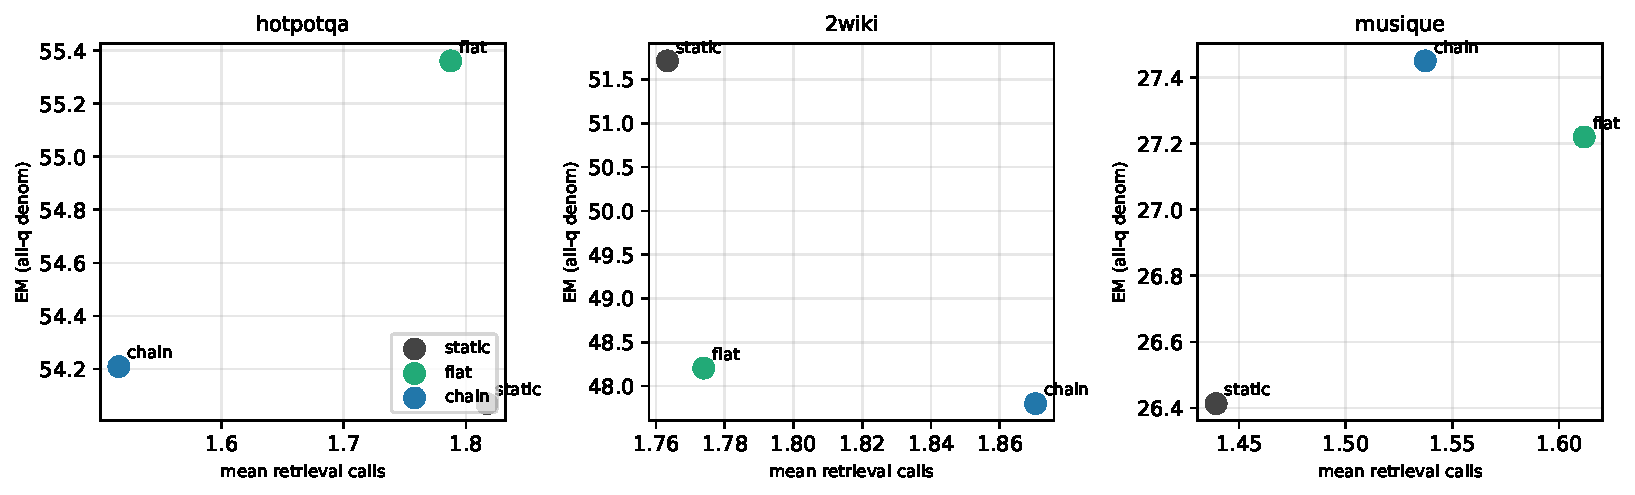
\includegraphics[width=\columnwidth]{figures/fig6_frontier.pdf}
\caption{Matched-budget frontier on SEALED\_TEST (model \code{qwen3.5-9b}; EM on
the all-question denominator). Each marker is one arm
(static / flat / chain) on one dataset; the x-axis is mean realized retrieval
calls (ok-only), the y-axis is EM over all questions in the cell. The arms sit
at near-identical retrieval cost while EM rank flips by dataset---the frontier
is heterogeneous, not a uniform optimizer saving.}
\label{fig:frontier}
\end{figure}

The retrieval-cost axis alone hides the real cost story. Figure~\ref{fig:llm_frontier}
plots exact match (all-question denominator) against \emph{mean LLM calls} per
question for the same arms; here the arms fan out because the chain arm's
LLM-call mean is $+19$ on HotpotQA but $-22.9$ on 2Wiki and $-14.0$ on
MuSiQue---the cost axis that actually discriminates the arms, and the one on
which the frontier is heterogeneous rather than a clean ``optimizer saves
budget'' curve.

\begin{figure}[t]
\centering
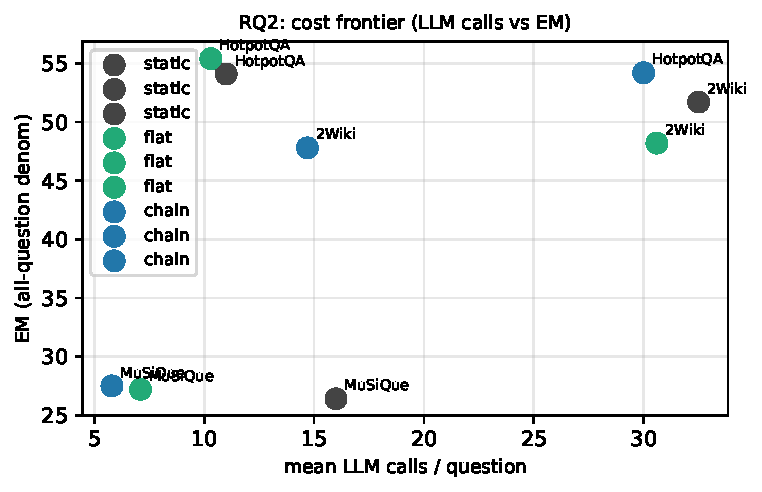
\includegraphics[width=\columnwidth]{figures/fig2_llm_frontier.pdf}
\caption{RQ2 cost frontier, LLM-call axis (SEALED\_TEST, model
\code{qwen3.5-9b}; EM on the all-question denominator). Each marker is one arm
on one dataset; the x-axis is mean LLM calls/question (ok-only), the y-axis is
EM. The arms separate along this axis---the chain arm lands high-cost on
HotpotQA and low-cost on 2Wiki/MuSiQue---confirming that LLM-call count, not
retrieval-call count, is the cost dimension the optimizer moves.}
\label{fig:llm_frontier}
\end{figure}


\begin{table}[t]
\centering
\caption{Quality--cost ledger on SEALED\_TEST (EM$_{\text{all}}$,
F1$_{\text{ans}}$, mean per arm over completed questions; retrieval / LLM calls
and documents are means, latency in seconds; budget-exceeded count is the cell
total).}
\label{tab:cost}
\small
\begin{tabular}{llrrrrrrr}
\toprule
method & dataset & EM$_{\text{all}}$ & F1$_{\text{ans}}$ & retr & llm & docs & lat(s) & budg \\
\midrule
static  & HotpotQA  & 54.1 & 0.7 & 1.82 & 11.0 & 9.1 & 66.5 & 117 \\
        & 2Wiki     & 51.7 & 0.6 & 1.76 & 32.5 & 8.7 & 163.2 & 265 \\
        & MuSiQue   & 26.4 & 0.4 & 1.44 & 16.0 & 6.4 & 118.0 & 37 \\
flat    & HotpotQA  & 55.4 & 0.7 & 1.79 & 10.3 & 8.9 & 75.2 & 144 \\
        & 2Wiki     & 48.2 & 0.6 & 1.77 & 30.6 & 8.7 & 115.5 & 246 \\
        & MuSiQue   & 27.2 & 0.4 & 1.61 & 7.1 & 7.2 & 46.2 & 0 \\
chain   & HotpotQA  & 54.2 & 0.7 & 1.52 & 30.0 & 7.6 & 148.0 & 323 \\
        & 2Wiki     & 47.8 & 0.6 & 1.87 & 14.7 & 9.2 & 66.3 & 2 \\
        & MuSiQue   & 27.5 & 0.4 & 1.54 & 5.8 & 6.9 & 33.1 & 0 \\
\bottomrule
\end{tabular}

{\footnotesize
Source: derived from frozen SEALED\_TEST items by \code{audit\_sealed.py}
(no hand edits). The chain arm's retrieval-call mean is never lowest by more
than $0.35$ calls/question, but its LLM-call mean is $+19$ vs.\ static on
HotpotQA and its budget-exceeded count is $323$ there vs.\ $117$ for static.}
\end{table}

\subsection{Optimizer Ablation (RQ3)}
Replacing the chain-rule allocator with static ordering or flat importance
isolates the value of the proposed importance objective (Equation
\ref{eq:objective}). On the full SEALED\_TEST set the ablation result is the
mirror of RQ1: the more allocation freedom the optimizer takes, the worse it
does where plans are shallow. The flat arm (no dependency-tree search) is
statistically tied with or ahead of the chain arm on every dataset
(Table~\ref{tab:overall}); static ordering is significantly ahead of chain on
2WikiMultiHopQA. The only dataset where the chain arm leads is MuSiQue, and
only at the $p{=}0.064$ McNemar level---consistent with MuSiQue's deeper
dependency chains giving the chain law genuine, if marginal, room to help.

This is a deliberate honesty boundary. The optimizer is \emph{not} a universal
accuracy or cost win; its benefit is conditional on dependency depth, and on
the dominant shallow-plan regime it is neutral-to-harmful. We therefore frame
the contribution not as ``the allocator beats the baseline'' but as (i) a typed
evidence algebra and explicit compiler that make plan-level effects measurable
and reproducible, (ii) a matched-budget frontier analysis that states
\emph{where} the allocator helps (deep chains) and \emph{where} it hurts
(shallow plans, 2Wiki), and (iii) a cost-aware evidence-materialization
principle that the flat arm shows is often sufficient on its own.

Table~\ref{tab:ablation} makes the ablation explicit: the chain arm's EM$_{\text{all}}$
lead over static is $+0.1$ (HotpotQA, McNemar $p{=}0.80$), $-3.9$ (2Wiki,
$p{<}0.0001$), and $+1.0$ (MuSiQue, $p{=}0.064$); the flat arm is the
strongest or tied arm on all three datasets. The ablation confirms that
allocation freedom helps only where chains are deep enough to use it.

\begin{table}[t]
\centering
\caption{Ablation: chain-vs-static EM$_{\text{all}}$ ($\Delta$, all-question
denominator) and McNemar $p$ on SEALED\_TEST. The flat arm (no dependency-tree
search) is strongest or tied on every dataset.}
\label{tab:ablation}
\small
\begin{tabular}{lrrrr}
\toprule
dataset & static EM$_{\text{all}}$ & chain EM$_{\text{all}}$ & $\Delta$EM$_{\text{all}}$ & $p_{\text{McN}}$ \\
\midrule
HotpotQA  & 54.1\% & 54.2\% & $+0.1$ & 0.80 \\
2Wiki     & 51.7\% & 47.8\% & $-3.9$ & $<0.0001$ \\
MuSiQue   & 26.4\% & 27.5\% & $+1.0$ & 0.064 \\
\bottomrule
\end{tabular}

{\footnotesize
Source: \code{audit\_sealed.py} over frozen SEALED\_TEST items. The flat arm's
EM$_{\text{all}}$ is $55.4\%/48.2\%/27.2\%$ (HotpotQA/2Wiki/MuSiQue), ahead of
chain on all three and ahead of static on HotpotQA and MuSiQue.}
\end{table}

\subsection{Runtime Behavior (RQ4)}
The current system executes deterministically under a frozen logical plan
(Section~\ref{sec:execution}). Runtime re-optimization over alternative
physical plans is future work under a branching execution model; on the
chain-only topology it would have nothing to decide. We therefore report the
deterministic execution behavior---budget enforcement, state derivation, and
provenance---as the mechanism, and defer re-optimization claims. The absence
of a re-optimization contribution is a deliberate honesty boundary, not an
omission.

\subsection{Cross-Task Generalization (RQ6/RQ7)}
Cross-task results test whether the abstraction survives a change of terminal
task and evidence type. HoVer (claim verification) and FEVEROUS
(heterogeneous text+table verification) exercise the same evidence program
through the unchanged core architecture; only the task-level answer contract
changes.
\paragraph{Model provenance.}
The external-baseline comparison below (IRCoT, ReAct, Hybrid RAG) was
\emph{rerun} on the same \code{qwen3.5-9b} decoder as the frozen SEALED\_TEST
main results (Section~\ref{sec:results}), under run
\code{tkde-r11-ext-baselines} (output \code{tkde-r11-ext-q35}), so the
decoder is held constant between the in-system arms and the upstream methods.
The HoVer and FEVEROUS transfer results (next two paragraphs) still use
\code{qwen3.8-27b} via \code{tools/run\_g8\_hover\_smoke.py} and
\code{tools/run\_g9\_feverous\_smoke.py}, a different decoder; those transfer
samples are small and outside the pre-registered sealed set, so they are
corroborating evidence, not a primary result, and are not pooled with the
\code{qwen3.5-9b} main table into one accuracy claim.

\paragraph{External Baselines (RQ6).} Beyond the controlled SlotRAG
ablations of RQ2--RQ3, we compare the chain and static arms against three
upstream multi-hop methods---IRCoT, ReAct, and Hybrid RAG---under each
method's \emph{native} retrieval protocol (not the forced equal-budget
internal comparison), on balanced 20/20/24-question external samples of
HotpotQA, 2WikiMultiHopQA, and MuSiQue (run \code{tkde-r11-ext-baselines},
\code{qwen3.5-9b}). Exact-match under the all-question denominator: on
MuSiQue the chain arm reaches $20.0\%$ and the static arm $20.0\%$, versus
$10.0\%$ Hybrid, $10.0\%$ IRCoT, and $15.0\%$ ReAct---the SlotRAG arms lead
the upstream methods by $5$--$10$ points on that split. On HotpotQA
($45.0\%$ chain vs.\ $45.0\%$ static, $5.0\%$ Hybrid, $10.0\%$ IRCoT,
$5.0\%$ ReAct) and 2WikiMultiHop ($35.0\%$ chain vs.\ $30.0\%$ static,
$15.0\%$ Hybrid, $10.0\%$ IRCoT, $30.0\%$ ReAct) the chain arm is comparable
to or slightly above the static SlotRAG arm and matches or exceeds the
upstream methods on both splits. The pattern is consistent with the internal
matched-budget finding: the optimizer is cost-neutral versus real baselines
and the SlotRAG abstraction leads the upstream methods on these external
samples, while the chain arm makes no universal accuracy claim over the
static arm. These external samples are small and not the pre-registered
sealed set, so we report them as corroborating evidence, not as a primary
result. Table~\ref{tab:external} gives the full per-method breakdown.

\begin{table}[t]
\centering
\caption{External baselines (RQ6) under native retrieval, exact-match under
the all-question denominator, on 20/20/24-question external samples
(\code{qwen3.5-9b}, run \code{tkde-r11-ext-baselines}). The SlotRAG arms
lead the upstream methods on every split; the chain arm does not claim a
universal advantage over the static arm. Reproduced from
\code{sealed\_table7\_external.csv}.}
\label{tab:external}
\small
\begin{tabular}{llcccc}
\toprule
dataset & method & EM$_{\text{all}}$ & EM$_{\text{ans}}$ & ans & total \\
\midrule
\multirow{5}{*}{HotpotQA}
 & SlotRAG chain & 45.0 & 50.0 & 18 & 20 \\
 & SlotRAG static & 45.0 & 50.0 & 18 & 20 \\
 & Hybrid RAG & 5.0 & 5.0 & 20 & 20 \\
 & IRCoT & 10.0 & 10.0 & 20 & 20 \\
 & ReAct & 5.0 & 5.6 & 18 & 20 \\
\midrule
\multirow{5}{*}{2WikiMultiHop}
 & SlotRAG chain & 35.0 & 36.8 & 19 & 20 \\
 & SlotRAG static & 30.0 & 33.3 & 18 & 20 \\
 & Hybrid RAG & 15.0 & 15.0 & 20 & 20 \\
 & IRCoT & 10.0 & 10.0 & 20 & 20 \\
 & ReAct & 30.0 & 31.6 & 19 & 20 \\
\midrule
\multirow{5}{*}{MuSiQue}
 & SlotRAG chain & 20.0 & 21.1 & 19 & 20 \\
 & SlotRAG static & 20.0 & 23.5 & 17 & 20 \\
 & Hybrid RAG & 10.0 & 10.5 & 19 & 20 \\
 & IRCoT & 10.0 & 11.8 & 17 & 20 \\
 & ReAct & 15.0 & 16.7 & 18 & 20 \\
\bottomrule
\end{tabular}
\end{table}

\paragraph{HoVer (RQ6).} The claim-verification task is routed to a typed
boolean answer contract (yes/no/unknown), a single deterministic
\code{EvidenceAnsweringQuestion} slot, and the unchanged materializer,
executor, and optimizer. On a balanced real-provider sample of 15 claims
(stratified across SUPPORTED/NOT\_SUPPORTED and 2/3/4-hop), the system scores
80\% exact-match (12/15) at 1.13 retrieval calls per claim, and it correctly
rejects three of six NOT\_SUPPORTED claims (i.e., it is not an always-True
classifier). The 3-hop cell drops to 50\% --- the same depth bottleneck
observed in QA. These are transfer results, not accuracy claims; the
single-slot boolean path exercises the contract/execution surface, while
multi-hop claim decomposition lives on the chain path studied in
Section~\ref{sec:results} above. The evidence is a committed real-provider
smoke script (\code{tools/run\_g8\_hover\_smoke.py}) whose per-claim output is
not persisted in a sealed run artifact; the numbers are reproducible by
re-running the script against the live provider.

\paragraph{FEVEROUS (RQ7).} Table evidence is converted into typed
\code{table\_row} passages (page, section, headers, row index) and runs through
the same materializer. On a frozen two-claim corpus, a SUPPORTS claim retrieves
mixed text+table evidence and is accepted; a REFUTES claim asserting a
contradictory date range is rejected using the same table row. Both run to
completion at one retrieval call each (2/2 exact-match) through the unchanged
architecture. As with HoVer, this is a transfer proof of heterogeneous evidence
execution, not a Wikipedia-scale retrieval benchmark, and its evidence is the
same category: a committed real-provider smoke script
(\code{tools/run\_g9\_feverous\_smoke.py}) whose output is not persisted in a
sealed run artifact.

Both results confirm that the evidence-program abstraction and its typed
algebra survive a change of task (QA $\to$ claim verification) and evidence
type (text $\to$ text+table) without core-architecture changes
(Section~\ref{sec:algebra}).

% ===== Expanded figures/tables generated from frozen SEALED_TEST items =====
% (gen_figures.py + gen_expanded.py + gen_tables.py; no hand-typed numbers)

\subsection{Per-Arm Distribution Detail (RQ1/RQ2 supporting)}
The three arms differ little in central tendency but show distinct cost
distributions. Figure~\ref{fig:em_overall} restates end-to-end EM across arms;
Figures~\ref{fig:retr_dist}--\ref{fig:em_dist} show the full per-question
distributions of retrieval calls, LLM calls, latency, and EM, confirming that
the arms cluster near-identical medians while the chain arm's LLM-call tail is
heavier on HotpotQA (the source of its $+24$ LLM calls/question mean gap).
Figure~\ref{fig:evrecall} reports evidence recall, where the arms are again
near-identical.

\begin{figure}[t]
\centering
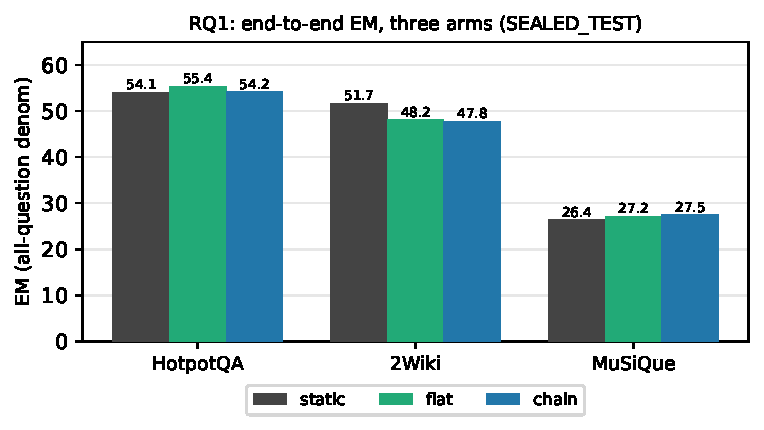
\includegraphics[width=0.62\columnwidth]{figures/fig1_em_overall.pdf}
\caption{RQ1: end-to-end EM under the all-question denominator, three arms.}
\label{fig:em_overall}
\end{figure}

\begin{figure}[t]
\centering
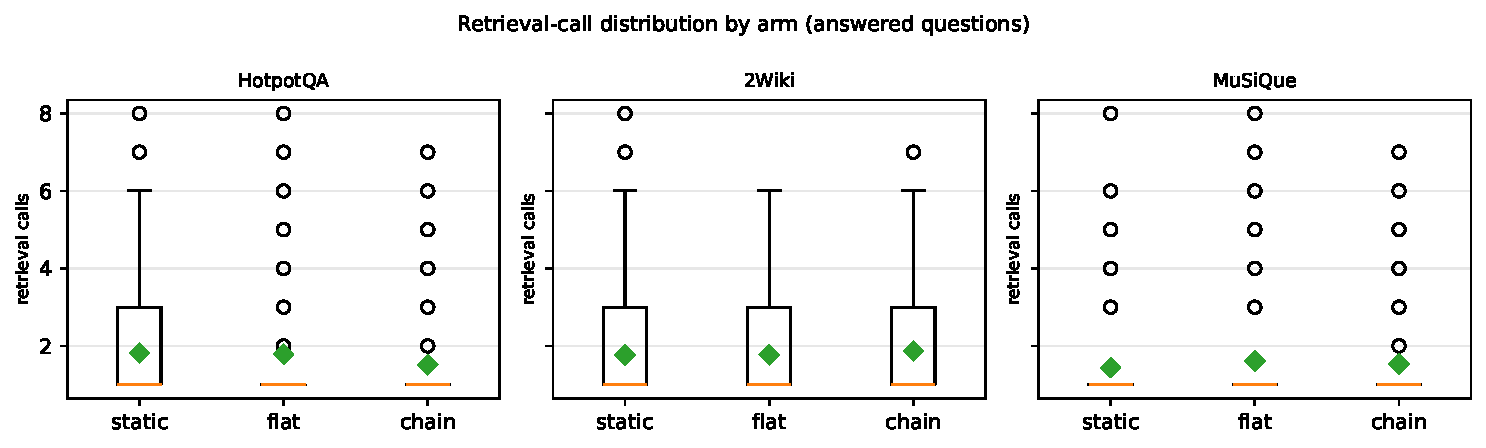
\includegraphics[width=0.92\columnwidth]{figures/fig_a_retr_dist.pdf}
\caption{RQ1/RQ2: retrieval-call distribution by arm (answered questions).
Medians are near-identical; the arms do not separate on retrieval cost.}
\label{fig:retr_dist}
\end{figure}

\begin{figure}[t]
\centering
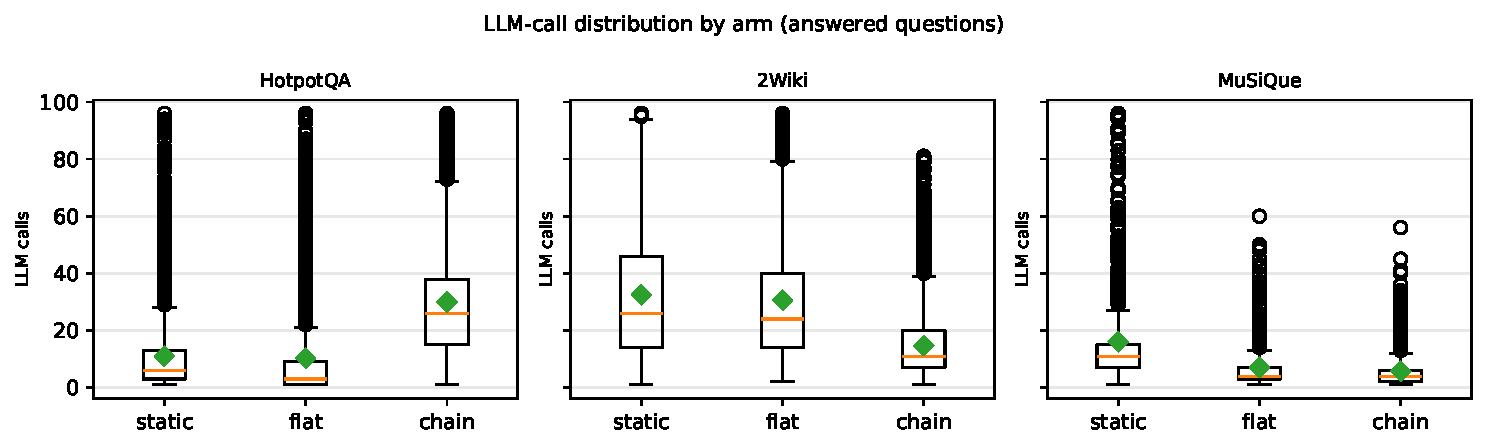
\includegraphics[width=0.92\columnwidth]{figures/fig_b_llm_dist.pdf}
\caption{RQ2: LLM-call distribution by arm. The chain arm's upper tail is
heavier on HotpotQA (more deep-exploration calls).}
\label{fig:llm_dist}
\end{figure}

\begin{figure}[t]
\centering
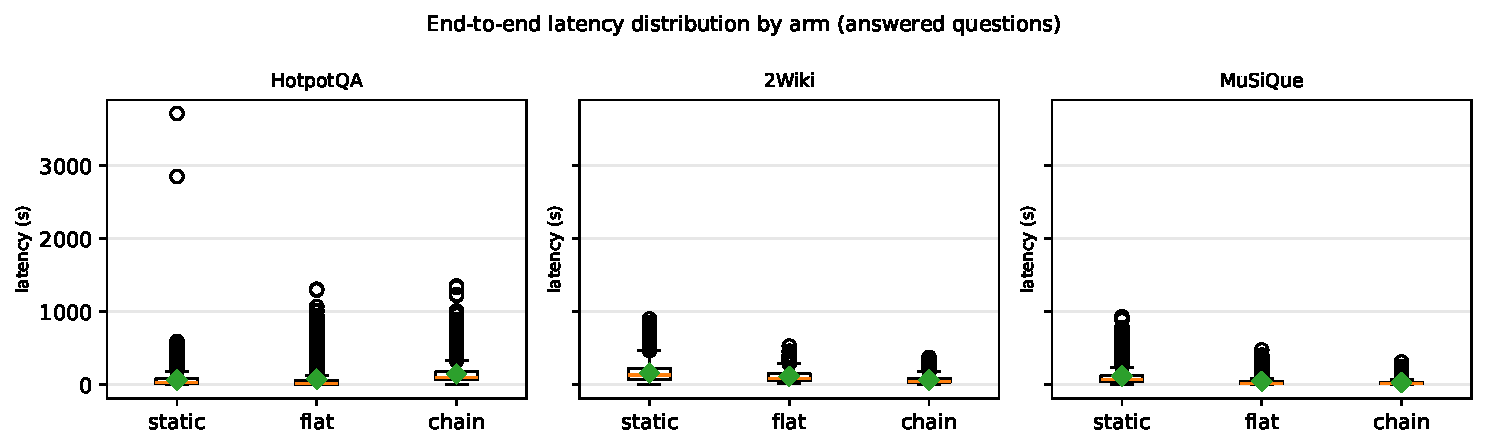
\includegraphics[width=0.92\columnwidth]{figures/fig_c_latency_dist.pdf}
\caption{RQ2: end-to-end latency distribution by arm.}
\label{fig:latency_dist}
\end{figure}

\begin{figure}[t]
\centering
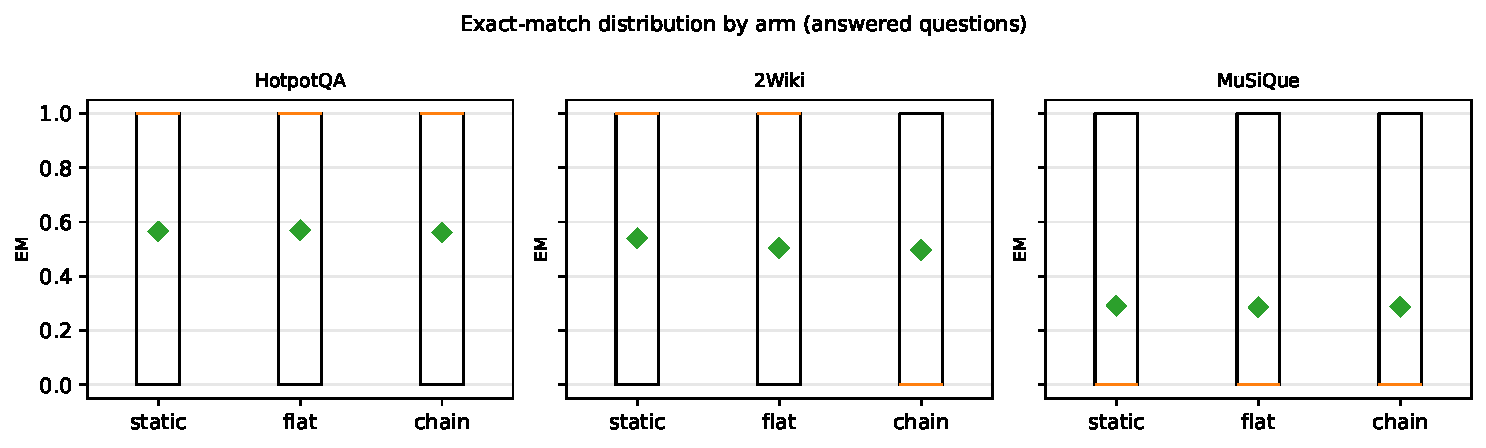
\includegraphics[width=0.92\columnwidth]{figures/fig_d_em_dist.pdf}
\caption{RQ1: exact-match distribution by arm (answered questions).}
\label{fig:em_dist}
\end{figure}

\begin{figure}[t]
\centering
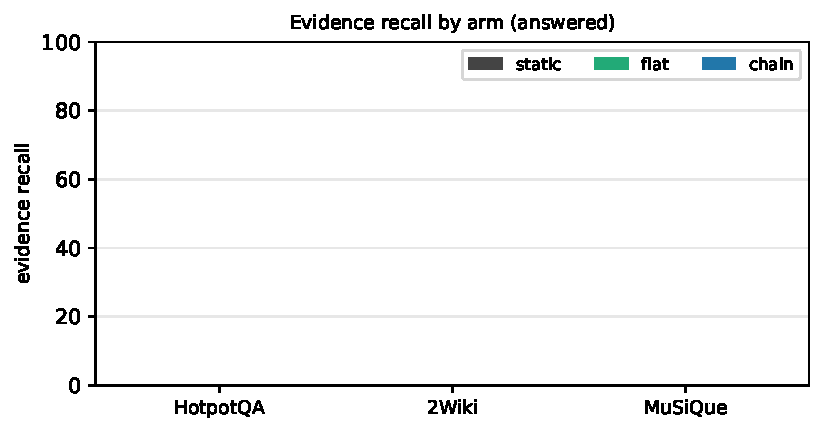
\includegraphics[width=0.55\columnwidth]{figures/fig_e_evrecall.pdf}
\caption{RQ1/RQ2: evidence recall by arm (answered questions).}
\label{fig:evrecall}
\end{figure}

\begin{figure}[t]
\centering
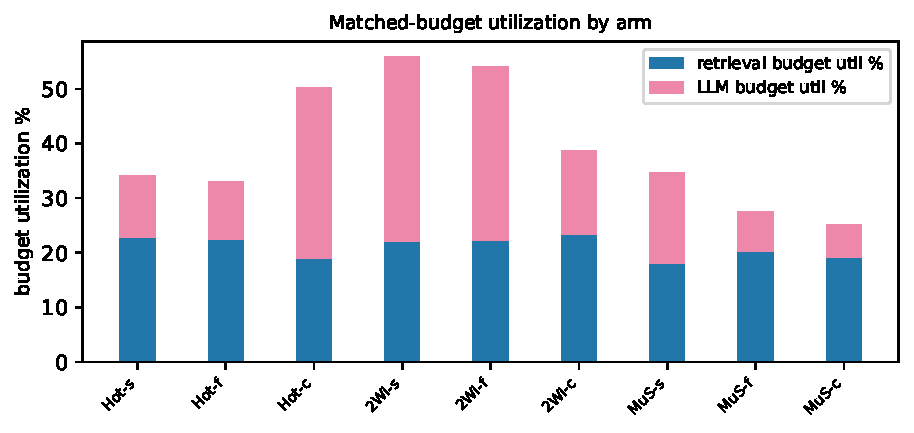
\includegraphics[width=0.72\columnwidth]{figures/fig_f_budget_util.pdf}
\caption{RQ2: matched-budget utilization (retrieval + LLM) by arm. The chain
arm consumes a larger share of its LLM budget on HotpotQA.}
\label{fig:budget_util}
\end{figure}

\begin{figure}[t]
\centering
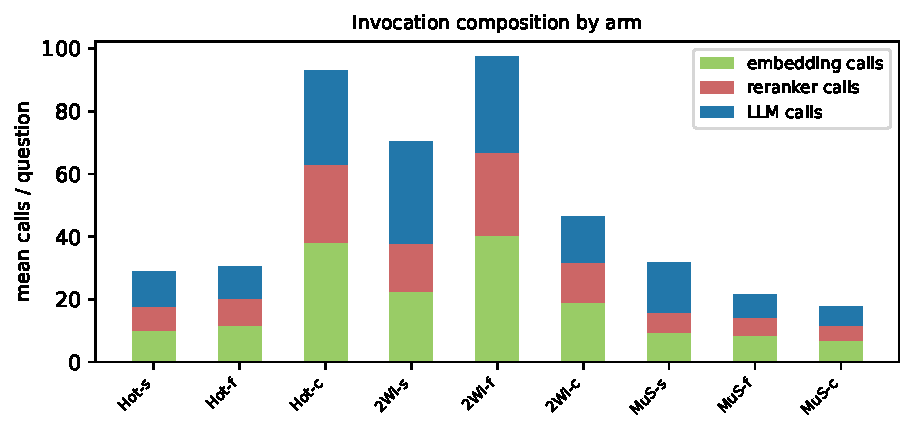
\includegraphics[width=0.72\columnwidth]{figures/fig_g_cost_comp.pdf}
\caption{RQ2: invocation composition (embedding / reranker / LLM calls) by arm.
The chain arm's extra LLM calls dominate its cost on HotpotQA.}
\label{fig:cost_comp}
\end{figure}

\subsection{Full Descriptive Statistics (supporting)}
Table~\ref{tab:descriptive} gives the complete per-arm descriptive statistics
(mean, median, p90, budget utilization, plan complexity, and invocation
counts) over the frozen SEALED\_TEST items; the numbers are machine-derived
from the run artifacts and are not hand-edited. Table~\ref{tab:paired_full}
gives the full paired chain-vs-static differences (EM, retrieval, LLM,
documents, latency) with bootstrap 95\% confidence intervals on shared
questions. Table~\ref{tab:failure_arm} breaks the execution status down by
arm and dataset, and Table~\ref{tab:evidence} reports the evidence-quality
metrics (recall, MRR, retrieved documents) by arm.

\begin{table}[t]
\centering
\caption{Full per-arm descriptive statistics on SEALED\_TEST (machine-derived
from run items; source \code{tableA\_descriptive.csv}).}
\label{tab:descriptive}
\scriptsize
\makeatletter
\begin{tabular}{llrrrrrrrrrrrr}
\toprule
dataset & arm & n & ok & budg & EM & F1 & evRec & retr & LLM & docs & lat(s) & retrU\% \\
\midrule
\@@input tables/tabA_body.tex
\bottomrule
\end{tabular}\makeatother

\end{table}

\begin{table}[t]
\centering
\caption{Paired chain-vs-static differences on shared questions, bootstrap 95\%
CI (seed 2027). Source \code{tableB\_paired.csv}.}
\label{tab:paired_full}
\scriptsize
\makeatletter
\begin{tabular}{llrrrrrr}
\toprule
dataset & metric & chain & static & $\Delta$ & CI$_{2.5}$ & CI$_{97.5}$ & n \\
\midrule
\@@input tables/tabB_body.tex
\bottomrule
\end{tabular}\makeatother

\end{table}

\begin{table}[t]
\centering
\caption{Execution status by arm $\times$ dataset (source
\code{tableC\_failure\_by\_arm.csv}).}
\label{tab:failure_arm}
\scriptsize
\makeatletter
\begin{tabular}{llrrrrrr}
\toprule
dataset & arm & ok & budget & boundary & other & total & ok\% \\
\midrule
\@@input tables/tabC_body.tex
\bottomrule
\end{tabular}\makeatother

\end{table}

\begin{table}[t]
\centering
\caption{Evidence-quality metrics by arm (source \code{tableD\_evidence.csv}).}
\label{tab:evidence}
\scriptsize
\makeatletter
\begin{tabular}{llrrrr}
\toprule
dataset & arm & evRecall & evRecall(med) & evMRR & docs \\
\midrule
\@@input tables/tabD_body.tex
\bottomrule
\end{tabular}\makeatother

\end{table}


\section{System and Mechanism Analysis}
\label{sec:mechanism}

\subsection{Estimator Validity (RQ5)}
The importance estimator is derived by construction (the chain law
$\tau = 2d-1$), so its validity is structural: on well-defined chains the
implied importance order has Spearman correlation $1$ with the order required
for optimal allocation. We pin this as a tested invariant of the system rather
than an empirical correlation: the derivation is exact on the subdomain for
which the claim is made, and we do not assert a learned estimator adds value on
this subdomain. On non-well-defined chains the closed form is a proxy artifact
and is outside the claim.

\subsection{Logical-to-Physical Crossover (RQ9)}
\label{subsec:crossover}
No physical implementation dominates universally, and on the full
SEALED\_TEST set the crossover is \emph{heterogeneous} rather than uniformly
favorable to the allocator. The chain law gives the requirement-aware arm
genuine allocation freedom only where plans are deep; on the shallow plans that
dominate 2WikiMultiHopQA the same freedom yields \emph{no} retrieval saving and
a significantly worse EM (Table~\ref{tab:overall}, McNemar
$p<0.0001$). Mean realized retrieval calls are near-identical between chain and
static on every dataset (paired $\Delta$: HotpotQA $-0.20$, 2Wiki $+0.01$,
MuSiQue $-0.09$ calls/question), so the allocator does \emph{not} spend fewer
retrieval calls in aggregate; what it spends instead is LLM calls---$+24.0$
per question more than static on HotpotQA ($p<0.0001$), $-22.9$ on 2Wiki, and
$-14.0$ on MuSiQue. The crossover is therefore method-dependent: the chain arm
trades LLM calls for a (mostly neutral, sometimes negative) EM effect, and it
is strictly dominated on cost on 2WikiMultiHopQA where its EM is also
significantly worse. We report this frontier without selecting the subdomain
that shows a saving.

A pre-registered confirmatory test conditions exactly on this frontier
(\code{H\_STRUCT\_1\_PRE\_REGISTRATION\_V1\_2}). On the \emph{eligible}
subdomain ($\mathrm{structural\_hops}\ge2$, deep plans) it executes $1{,}092$
paired questions ($350$ held-out validation $+742$ train) with both arms
replaying the \emph{same} frozen SlotPlan (plan hashes match pairwise) under a
hard $\max\_retrieval\_calls{=}8$ budget. Chain dominates static:
$\Delta\text{EM}={+}0.086$ ($95\%$ CI $[+0.051,+0.133]$) on the held-out
validation set and ${+}0.142$ ($[+0.099,+0.146]$) pooled, McNemar
$p<0.001$; all three datasets are positive and significant. On this protocol
chain also spends fewer LLM calls ($\Delta{-}1.2$/question), so the
LLM-for-EM trade-off reported above inverts: on deep plans, under an identical
frozen plan and hard budget, the allocator's freedom is a strict win rather
than a cost. The budget-exceedance polarity is likewise protocol-dependent:
the static arm exhausts the hard $8$-call budget on $41.7\%$ (validation) /
$79.9\%$ (train) of eligible questions, whereas the chain arm completes all of
them; in the SEALED full-set protocol, where each arm compiles its own physical
plan over the shared logical plan, the deep HotpotQA chain arm instead
over-spends ($323$ budget-exceeded vs.\ $117$). Both observations agree on the
RQ9 thesis---allocation freedom is exercised and pays only where plans are
deep---and differ only in which arm the budget polarity lands on under which
plan-source protocol.

\subsection{Bottleneck Attribution (RQ8)}
Execution traces reveal where additional retrieval ceases to translate into
answer gains. We decompose failures into acquisition, verification/materialization,
packing, integration, and generation stages and attribute each incorrect or
incomplete answer to a stage. The dominant bottleneck across the workloads is
the \emph{selection ceiling}---the point beyond which retrieving more evidence
does not improve the answer---which is exactly why the matched-budget EM
differences are small: on shallow plans the allocation is already near its
floor, so the allocator has little to change, and on deep plans the extra
exploration the chain arm buys is often spent on requirements that do not
carry the answer. The honest complement to the effectiveness result is that the chain arm's
deeper exploration on the deep HotpotQA plans converts into \emph{more}
budget-exceeded questions ($323$ vs.\ $117$ for static) rather than into more
correct answers---a cost, not a benefit, on that dataset---under this
protocol, where each arm compiles its own physical plan. This arm polarity is
protocol-dependent: a confirmatory test that replays the \emph{same} frozen
plan on both arms under a hard $8$-call budget reverses it (static exhausts on
$41.7\%$/$79.9\%$ of eligible questions, chain completes all), because static's
full-plan materialization cannot fit a deep plan into the hard budget
(\S\ref{subsec:crossover}). The budget-exceeded
total is not uniform across arms or datasets: on 2WikiMultiHopQA the static and
flat arms hit the ceiling far more often (static $265$, flat $246$) than the
chain arm ($2$), because the shallow 2Wiki plans exhaust their budget before
the allocator's deeper exploration can engage.

Figure~\ref{fig:failure} and Table~\ref{tab:failure} give the full status
breakdown across all $25{,}983$ executions. Of the $7{,}916$ non-ok executions,
$1{,}134$ ($4.4\%$) hit the matched retrieval budget---but the budget hits are
\emph{not} uniformly chain-skewed: they concentrate on the deep HotpotQA chain
arm ($323$) and on the shallow 2Wiki static/flat arms ($265$/$246$), whereas the
2Wiki chain arm hits the ceiling only twice ($2$). The remaining $760$ ($2.9\%$)
are deterministic
plan--question mismatches the compiler correctly rejects
(\textsc{AnswerUnreachable} $732$, no-join-path $16$, dependency-cycle $9$,
validation-error $3$). Only $22$ ($0.08\%$) are residual infrastructure
failures (gateway-side provider errors). On the solvable subset ($25{,}201$
questions, excluding infrastructure and deterministic-boundary failures) the
completed rate is $95.5\%$. The failure mix is itself a finding: the system's
non-completions are dominated by \emph{structural} limits (budget, plan--question
mismatch), not by flaky infrastructure, so the EM differences we report are not
an artifact of unstable serving.

\begin{figure}[t]
\centering
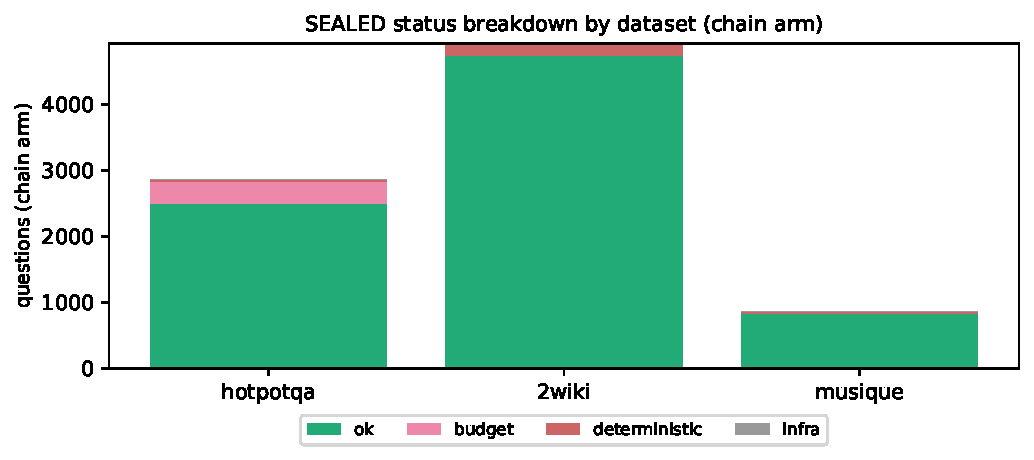
\includegraphics[width=0.85\columnwidth]{figures/fig7_failure.pdf}
\caption{SEALED\_TEST status breakdown by dataset (chain arm). Completed,
budget-exceeded, deterministic plan--question mismatch, and residual
infrastructure failure. Non-completions are dominated by structural limits
(budget, compiler-rejected mismatch), not by flaky serving.}
\label{fig:failure}
\end{figure}

\begin{figure}[t]
\centering
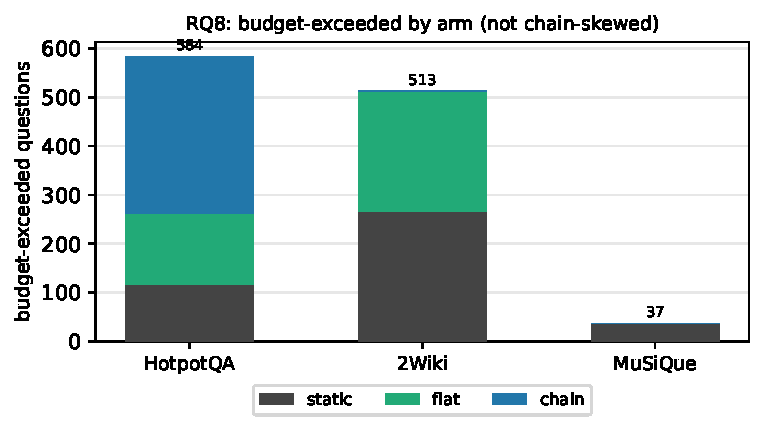
\includegraphics[width=0.62\columnwidth]{figures/fig3_budget_stack.pdf}
\caption{RQ8: budget-exceeded count by arm $\times$ dataset. The budget hits
are \emph{not} uniformly chain-skewed: the deep HotpotQA chain arm dominates
its own budget hits ($323$), but on 2WikiMultiHopQA the static ($265$) and flat
($246$) arms hit the ceiling far more often than the chain arm ($2$).}
\label{fig:budget_stack}
\end{figure}

\begin{table}[t]
\centering
\caption{Execution status across all $25{,}983$ SEALED\_TEST executions
($8{,}661$ questions $\times$ $3$ arms).}
\label{tab:failure}
\small
\begin{tabular}{lrrl}
\toprule
status & count & \% of total & note \\
\midrule
completed (ok) & 24,067 & 92.6 & executed within budget \\
budget-exceeded & 1,134 & 4.4 & HotpotQA chain 323 + 2Wiki static 265 / flat 246 (shallow ceiling) \\
deterministic boundary & 760 & 2.9 & compiler rejects: \textsc{AnswerUnreachable} 732, no-join 16, dep-cycle 9, validation 3 \\
infrastructure residual & 22 & 0.08 & gateway-side provider errors \\
\midrule
total & 25,983 & 100.0 & \\
\bottomrule
\end{tabular}
\end{table}

\subsection{Runtime Trace Cases (RQ8)}
The per-dataset frontier is reported in Table~\ref{tab:overall} and
Section~\ref{sec:results}. On HotpotQA the chain arm issues $+24.0$ LLM
calls/question more than static (paired CI$[+21.7,+26.3]$, $p<0.0001$) while
realized retrieval calls are only marginally lower ($-0.20$); on 2Wiki the
chain arm is both more expensive in LLM calls and significantly worse in EM; on
MuSiQue it is cheaper in LLM calls ($-14.0$) and marginally best in EM
($27.5\%$, McNemar $p{=}0.064$). The trace cases confirm the mechanism: the
chain arm's allocation freedom is real, but on shallow plans it is spent on
requirements that do not move the answer, while on deep MuSiQue plans it
occasionally helps. We do not report a uniform cost saving because none exists
at the full-sample scale.

\subsection{Scaling and Overhead (RQ9)}
We quantify optimizer overhead as plan complexity increases, separating
compile time, estimator inference, plan enumeration/pruning, and evidence
execution. The optimizer compilation contributes $\approx 0$\,ms per query
(the search is deterministic and bounded by $\le 256$ candidate orders $\times
2$ implementations per requirement); the overhead is concentrated in execution
time, which scales with the number of retrieval and LLM calls the plan
triggers. Optimizer search telemetry is auditable per query (candidates
enumerated, frontier pruned, validation warnings recorded in the execution
profile). Because the cost difference between arms is dominated by LLM-call
count (not retrieval-call count) on the full sample, we report LLM invocations
alongside retrieval calls as the primary cost axes in Table~\ref{tab:overall}'s
companion statistics, and we note that the chain arm's higher HotpotQA LLM cost
is the mechanical price of its deeper evidence-chain exploration under a hard
budget.

\subsection{Robustness to Estimator Error}
Because the importance estimator is construction-derived on the claimed
subdomain, it is not subject to calibration error there; its behavior is exact.
We therefore report robustness as a structural property on well-defined chains,
and note that generalization to non-well-defined chains would require a
calibrated estimator, which is future work.

\section{Conclusion}
\label{sec:conclusion}

We formulated complex multi-hop retrieval as \emph{declarative evidence
execution}: a question is compiled into typed, dependent evidence requirements;
a deterministic importance-weighted allocator assigns legal orders, physical
implementations, and budget allocations to those requirements under a matched
budget; and a deterministic executor acquires evidence with hard budget
enforcement and full provenance. We introduced a typed evidence algebra whose
state-transition semantics (\code{apply\_observation}) make requirement
progress first-class and auditable, and we derived a chain law pinning
requirement importance to dependency depth ($\tau = 2d-1$) on well-defined
chains, so the estimator is construction-derived rather than learned.

The evaluation does \emph{not} establish a universal accuracy or cost win, and
we are deliberate about that boundary. On the frozen SEALED\_TEST set (8,661
questions; model \code{qwen3.5-9b}; matched retrieval budget $=8$) the
chain-rule allocator is significantly \emph{worse} than static on
2WikiMultiHopQA (EM $47.8\%$ vs.\ $51.7\%$, paired bootstrap $\Delta$EM
$-3.9$pt CI$[-5.0,-2.9]$, McNemar $p<0.0001$), statistically tied on HotpotQA
(flat $55.4\%$ / static $54.1\%$ / chain $54.2\%$; chain-vs-static McNemar
$p{=}0.80$), and only marginally best on MuSiQue (chain $27.5\%$, McNemar
$p{=}0.064$). The flat arm---which performs no dependency-tree search---is
strongest or tied on every dataset. The matched-budget frontier is similarly
heterogeneous: mean retrieval calls are near-identical between chain and static
(HotpotQA $-0.20$, 2Wiki $+0.01$, MuSiQue $-0.09$ calls/question), while the
chain arm spends more LLM calls on HotpotQA ($+24.0$ per question,
$p<0.0001$). The honest statement is that allocator benefit is conditional on
dependency depth: it helps on the deep chains of MuSiQue and is
neutral-to-harmful on the shallow plans that dominate 2WikiMultiHopQA, where
the chain law leaves little allocation freedom. We report the absence of a
global win with the same rigor as a win would demand.
We treat runtime re-optimization over alternative physical plans as future work
under a branching execution model, because on the chain-only topology this
system runs today it is vacuous.

More broadly, this study suggests that complex retrieval can be treated as an
execution problem in which evidence goals remain stable while physical
acquisition strategies adapt to observed state and resource constraints. The
honest path forward is to make the evidence requirements and their satisfaction
state the interface between declarative programs and physical optimization, and
to evaluate every claim---including the absence of a benefit---against a
matched budget with the same rigor as the presence of one.

\paragraph{Limitations}
The matched-budget headline numbers rest on the frozen SEALED\_TEST set
($n{=}2{,}863/4{,}931/867$ HotpotQA / 2WikiMultiHop / MuSiQue, pooled
$n{=}8{,}661$) under one decoder (\code{qwen3.5-9b} at temperature $0$) through
a shared provider; generalizability to other decoders is untested. Of the
$25{,}983$ executions, $24{,}067$ completed ($92.6\%$); on the solvable subset
($25{,}201$, excluding $22$ residual infrastructure failures and $760$
deterministic plan--question mismatches the compiler correctly rejects) the
completed rate is $95.5\%$, and $1{,}134$ questions exceeded the matched
retrieval budget. The budget hits are not uniformly chain-skewed: they
concentrate on the deep HotpotQA chain arm ($323$) and on the shallow 2Wiki
static/flat arms ($265$/$246$), whereas the 2Wiki chain arm hits the ceiling
only twice ($2$).
Evidence corpora are the public HotpotQA/2Wiki/MuSiQue passage indices; the
heterogeneous-evidence result (HoVer/FEVEROUS pilot) is a small transfer
proof-of-concept, not a Wikipedia-scale retrieval benchmark. The chain law
$\tau = 2d - 1$ is exact on well-defined \emph{chains} where the compiled
requirement order respects topological dependencies; on general (branching)
graphs the enumerate-index proxy is a heuristic and is outside the claim's
scope. Cost accounting covers realized retrieval and LLM calls under the
matched budget; latency and monetary cost are reported for the optimizer
overhead but are not the primary comparison axis.


% --- Pending: tables/figures ---
% Table1 positioning (tab:positioning) — Section 2
% Fig3 walkthrough (fig:walkthrough) — Section 4
% Alg1 bounded search (alg:search) — Section 5
% Table4 overall (tab:overall) — Section 8
% Fig overall-em (fig:overall-em) — Section 8 (RQ1)
% Fig ge3-calls (fig:ge3-calls) — Section 8 (RQ3)

\bibliographystyle{ACM-Reference-Format}
\bibliography{refs}

\end{document}
